\section{Assumptions}

This thesis posits that enduring, high-level musical elements persist regardless of sonic changes and constantly evolve within their context, mirroring the nature of sheet music's symbolic domain. A single waveform can correspond to a finite set of representations, but one music piece can yield infinite interpretations, varying by factors such as instruments and performance styles.

The premise of our work is that regardless of the waveform or production style, abstract high-level features can be discerned, offering objective and thorough insight into a composition's musical content, analogous to analyzing sheet music for its basic behaviors.

These characteristics aid listeners in recognizing and recreating musical structures, promoting deeper interaction with music. Mental shortcuts or heuristics enable a swift understanding of complex musical notions, revealing underlying patterns.

Despite differing cultural contexts, styles, time and key signatures, and sonic properties, we suggest a commonality between figures \ref{fig:mahler} and \ref{fig:giant_steps}. Both pieces display the same 'musicological flavour,' derived from their melodic and harmonic contour envelopes through non-diatonic major thirds.

This concept aligns with the theories of Kurt Koffka, a founding member of the Gestalt school of psychology, who advocated for a holistic approach to understanding complex forms, as opposed to the structuralist practice of dissecting mental processes into their elemental components \cite{Koffka2013PrinciplesPsychology}. In the context of music, Gestalt psychology principles suggest our minds process auditory input similarly to visual input by seeking patterns and structures. This understanding significantly enhances the comprehension of cognitive processes in musical perception and organization, influencing music theory, cognition, and therapy \cite{Lerdahl1985AMusic}.

\begin{figure}[ht]
    \centering
    \scalebox{0.9}{
    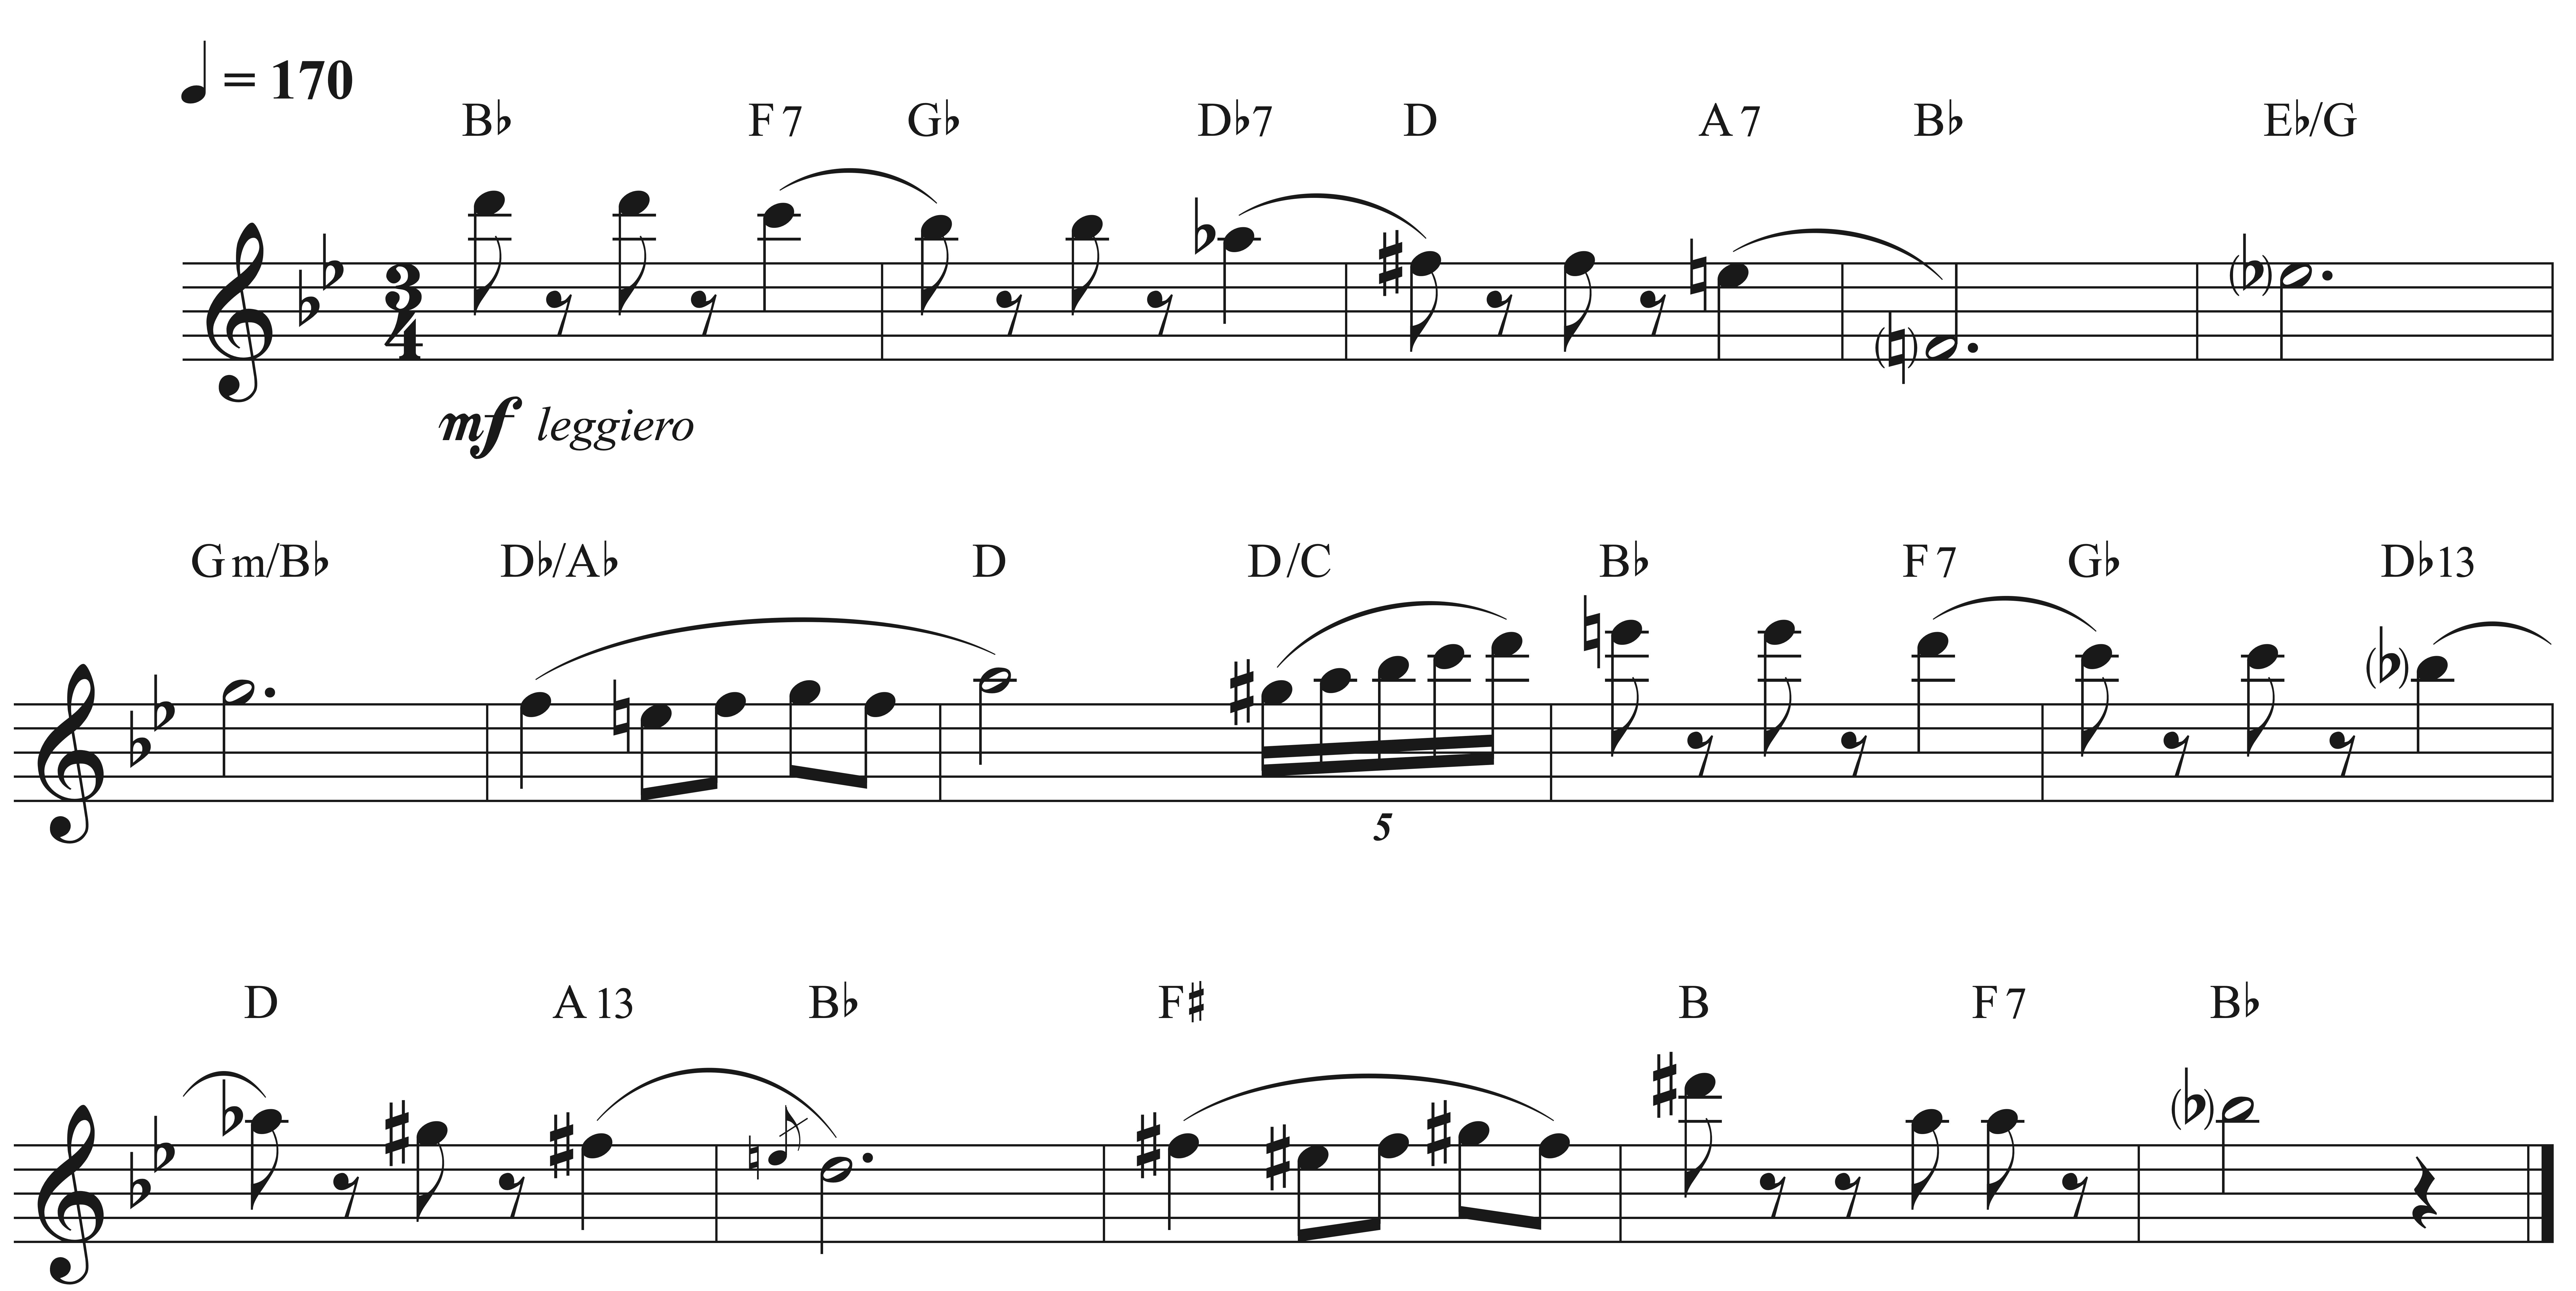
\includegraphics[width=\textwidth]{figures/images/Mahler 9 Giant Steps score.png}
        }
    \caption[Mahler's 9th Symphony, 2nd movement]{\small{A small excerpt from Mahler's 9th Symphony, 2nd movement: The melodic and harmonic contour propels through non-diatonic major thirds.}}
    \label{fig:mahler}
\end{figure}

\begin{figure}[ht]
    \centering
    \scalebox{0.9}{
    \includegraphics[width=\textwidth]{figures/images/giant steps score.png}
        }
    \caption[Giant Steps]{\small{John Coltrane's Giant Steps head: A testament to harmonic exploration, featuring rapid chord changes in non-diatonic major thirds.}}
    \label{fig:giant_steps}
\end{figure}
